\documentclass[tikz,border=5pt]{standalone}

\usepackage{amsmath,amsfonts,bm,graphicx}
\usepackage{tikz}
\usetikzlibrary{arrows.meta}

% Define your colors/macros here
\definecolor{cregmean}{RGB}{213,55,50}
\definecolor{cactmat}{RGB}{0,158,115}
\definecolor{cgray}{gray}{0.45}
\colorlet{cregmeanfill}{cregmean!15}
\colorlet{cactmatfill}{cactmat!15}
\colorlet{cgrayfill}{gray!15}

\newcommand{\figfont}{\footnotesize}
\newcommand{\figtitlefont}{\sffamily\bfseries\small}
\newcommand{\methodname}{ACTMat}
\newcommand{\modelcardlabel}{\resizebox{0.82cm}{!}{$\mW_1\!\cdots\!\mW_T$}}
\newcommand{\mergedlabel}{\resizebox{0.50cm}{!}{$\mW^\ast$}}
\newcommand{\mW}{\bm{W}}
\newcommand{\mC}{\bm{C}}
\newcommand{\mDelta}{\bm{\Delta}}
\newcommand{\vz}{\bm{z}}
\newcommand{\E}{\mathbb{E}}
\colorlet{cred}{cregmean}

\begin{document}

% regmean-vs-eigcov.tex
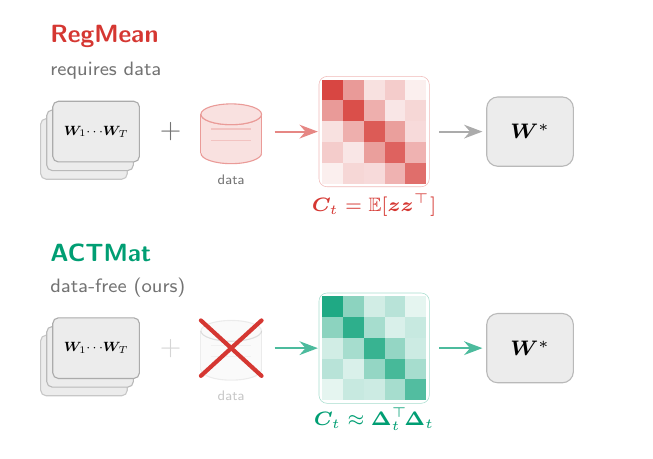
\begin{tikzpicture}[
    >=Stealth,
    scale=1.1, % Adjust this until it fits your 0.45\linewidth
    every node/.style={font=\figfont}
]
\path[use as bounding box] (-0.15, -0.55) rectangle (6.75, 4.10);

% === RegMean row ===
\node[anchor=west, font=\figtitlefont, text=cregmean] at (0, 4.0) {RegMean};
\node[anchor=west, font=\sffamily\scriptsize, text=cgray] at (0, 3.6) {requires data};

% Stacked model cards
\fill[cgrayfill, draw=cgray!40, rounded corners=2pt] (0.0, 2.35) rectangle ++(1.0, 0.7);
\fill[cgrayfill, draw=cgray!50, rounded corners=2pt] (0.07, 2.45) rectangle ++(1.0, 0.7);
\fill[cgrayfill, draw=cgray!60, rounded corners=2pt] (0.14, 2.55) rectangle ++(1.0, 0.7);
\node[inner sep=0pt] at (0.64, 2.9) {\modelcardlabel};

% Plus sign between weights and data
\node[font=\sffamily\bfseries, text=cgray] at (1.5, 2.9) {$+$};

% Data cylinder icon
\begin{scope}[shift={(1.85, 2.55)}]
    \fill[cregmeanfill] (0, 0.1) -- (0, 0.55) arc[start angle=180, end angle=360, x radius=0.35, y radius=0.12] -- (0.7, 0.1) arc[start angle=0, end angle=-180, x radius=0.35, y radius=0.12];
    \draw[cregmean!50] (0, 0.1) -- (0, 0.55);
    \draw[cregmean!50] (0.7, 0.1) -- (0.7, 0.55);
    \draw[cregmean!50] (0, 0.55) arc[start angle=180, end angle=360, x radius=0.35, y radius=0.12];
    \fill[cregmeanfill] (0, 0.55) arc[start angle=180, end angle=0, x radius=0.35, y radius=0.12] arc[start angle=0, end angle=-360, x radius=0.35, y radius=0.12];
    \draw[cregmean!50] (0.35, 0.55) ellipse[x radius=0.35, y radius=0.12];
    \draw[cregmean!50] (0, 0.1) arc[start angle=180, end angle=360, x radius=0.35, y radius=0.12];
    \draw[cregmean!30] (0.12, 0.38) -- (0.58, 0.38);
    \draw[cregmean!30] (0.12, 0.25) -- (0.58, 0.25);
\end{scope}
\node[font=\sffamily\tiny, text=cgray] at (2.2, 2.35) {data};

% Arrow to heatmap
\draw[->, cregmean!60, thick] (2.7, 2.9) -- (3.2, 2.9);

% Red heatmap 5x5 for C_t
\begin{scope}[shift={(3.25, 2.3)}]
    \clip[rounded corners=3pt] (-0.04, -0.04) rectangle (1.24, 1.24);
    \fill[white] (-0.04, -0.04) rectangle (1.24, 1.24);
    \fill[cregmean, opacity=0.92] (0.00, 0.96) rectangle ++(0.24, 0.24);
    \fill[cregmean, opacity=0.50] (0.24, 0.96) rectangle ++(0.24, 0.24);
    \fill[cregmean, opacity=0.15] (0.48, 0.96) rectangle ++(0.24, 0.24);
    \fill[cregmean, opacity=0.25] (0.72, 0.96) rectangle ++(0.24, 0.24);
    \fill[cregmean, opacity=0.08] (0.96, 0.96) rectangle ++(0.24, 0.24);
    \fill[cregmean, opacity=0.50] (0.00, 0.72) rectangle ++(0.24, 0.24);
    \fill[cregmean, opacity=0.88] (0.24, 0.72) rectangle ++(0.24, 0.24);
    \fill[cregmean, opacity=0.40] (0.48, 0.72) rectangle ++(0.24, 0.24);
    \fill[cregmean, opacity=0.12] (0.72, 0.72) rectangle ++(0.24, 0.24);
    \fill[cregmean, opacity=0.20] (0.96, 0.72) rectangle ++(0.24, 0.24);
    \fill[cregmean, opacity=0.15] (0.00, 0.48) rectangle ++(0.24, 0.24);
    \fill[cregmean, opacity=0.40] (0.24, 0.48) rectangle ++(0.24, 0.24);
    \fill[cregmean, opacity=0.82] (0.48, 0.48) rectangle ++(0.24, 0.24);
    \fill[cregmean, opacity=0.48] (0.72, 0.48) rectangle ++(0.24, 0.24);
    \fill[cregmean, opacity=0.18] (0.96, 0.48) rectangle ++(0.24, 0.24);
    \fill[cregmean, opacity=0.25] (0.00, 0.24) rectangle ++(0.24, 0.24);
    \fill[cregmean, opacity=0.12] (0.24, 0.24) rectangle ++(0.24, 0.24);
    \fill[cregmean, opacity=0.48] (0.48, 0.24) rectangle ++(0.24, 0.24);
    \fill[cregmean, opacity=0.78] (0.72, 0.24) rectangle ++(0.24, 0.24);
    \fill[cregmean, opacity=0.38] (0.96, 0.24) rectangle ++(0.24, 0.24);
    \fill[cregmean, opacity=0.08] (0.00, 0.00) rectangle ++(0.24, 0.24);
    \fill[cregmean, opacity=0.20] (0.24, 0.00) rectangle ++(0.24, 0.24);
    \fill[cregmean, opacity=0.18] (0.48, 0.00) rectangle ++(0.24, 0.24);
    \fill[cregmean, opacity=0.38] (0.72, 0.00) rectangle ++(0.24, 0.24);
    \fill[cregmean, opacity=0.72] (0.96, 0.00) rectangle ++(0.24, 0.24);
    \draw[cregmean!35, rounded corners=3pt] (-0.04, -0.04) rectangle (1.24, 1.24);
\end{scope}
\node[font=\sffamily\scriptsize, text=cregmean] at (3.85, 2.05) 
{$\mC_t = \E[\vz\vz^\top]$};

% Arrow to W*
\draw[->, cgray!60, thick] (4.6, 2.9) -- (5.1, 2.9);

% Merged W*
\fill[cgrayfill, draw=cgray!50, rounded corners=4pt] (5.15, 2.5) rectangle ++(1.0, 0.8);
\node[inner sep=0pt] at (5.65, 2.9) {\mergedlabel};


% === \methodname row ===
\node[anchor=west, font=\figtitlefont, text=cactmat] at (0, 1.5) {\methodname};
\node[anchor=west, font=\sffamily\scriptsize, text=cgray] at (0, 1.1) {data-free (ours)};

% Stacked model cards
\fill[cgrayfill, draw=cgray!40, rounded corners=2pt] (0.0, -0.15) rectangle ++(1.0, 0.7);
\fill[cgrayfill, draw=cgray!50, rounded corners=2pt] (0.07, -0.05) rectangle ++(1.0, 0.7);
\fill[cgrayfill, draw=cgray!60, rounded corners=2pt] (0.14, 0.05) rectangle ++(1.0, 0.7);
\node[inner sep=0pt] at (0.64, 0.4) {\modelcardlabel};

% Plus sign (faded to match ghosted cylinder)
\node[font=\sffamily\bfseries, text=cgray!30] at (1.5, 0.4) {$+$};

% Ghosted data cylinder — same position as RegMean's but faded
\begin{scope}[shift={(1.85, 0.05)}, opacity=0.25]
    \fill[cgrayfill] (0, 0.1) -- (0, 0.55) arc[start angle=180, end angle=360, x radius=0.35, y radius=0.12] -- (0.7, 0.1) arc[start angle=0, end angle=-180, x radius=0.35, y radius=0.12];
    \draw[cgray!50] (0, 0.1) -- (0, 0.55);
    \draw[cgray!50] (0.7, 0.1) -- (0.7, 0.55);
    \draw[cgray!50] (0, 0.55) arc[start angle=180, end angle=360, x radius=0.35, y radius=0.12];
    \fill[cgrayfill] (0, 0.55) arc[start angle=180, end angle=0, x radius=0.35, y radius=0.12] arc[start angle=0, end angle=-360, x radius=0.35, y radius=0.12];
    \draw[cgray!50] (0.35, 0.55) ellipse[x radius=0.35, y radius=0.12];
    \draw[cgray!50] (0, 0.1) arc[start angle=180, end angle=360, x radius=0.35, y radius=0.12];
    \draw[cgray!30] (0.12, 0.38) -- (0.58, 0.38);
    \draw[cgray!30] (0.12, 0.25) -- (0.58, 0.25);
\end{scope}
\node[font=\sffamily\tiny, text=cgray!40] at (2.2, -0.15) {data};
% Red X over ghosted cylinder
\draw[cred, line width=1.5pt, line cap=round] (1.85, 0.08) -- (2.55, 0.72);
\draw[cred, line width=1.5pt, line cap=round] (2.55, 0.08) -- (1.85, 0.72);

% Arrow from weights to heatmap
\draw[->, cactmat!70, thick] (2.7, 0.4) -- (3.2, 0.4);

% Green heatmap 5x5 for Delta^T Delta
\begin{scope}[shift={(3.25, -0.2)}]
    \clip[rounded corners=3pt] (-0.04, -0.04) rectangle (1.24, 1.24);
    \fill[white] (-0.04, -0.04) rectangle (1.24, 1.24);
    \fill[cactmat, opacity=0.88] (0.00, 0.96) rectangle ++(0.24, 0.24);
    \fill[cactmat, opacity=0.45] (0.24, 0.96) rectangle ++(0.24, 0.24);
    \fill[cactmat, opacity=0.18] (0.48, 0.96) rectangle ++(0.24, 0.24);
    \fill[cactmat, opacity=0.28] (0.72, 0.96) rectangle ++(0.24, 0.24);
    \fill[cactmat, opacity=0.10] (0.96, 0.96) rectangle ++(0.24, 0.24);
    \fill[cactmat, opacity=0.45] (0.00, 0.72) rectangle ++(0.24, 0.24);
    \fill[cactmat, opacity=0.82] (0.24, 0.72) rectangle ++(0.24, 0.24);
    \fill[cactmat, opacity=0.35] (0.48, 0.72) rectangle ++(0.24, 0.24);
    \fill[cactmat, opacity=0.15] (0.72, 0.72) rectangle ++(0.24, 0.24);
    \fill[cactmat, opacity=0.22] (0.96, 0.72) rectangle ++(0.24, 0.24);
    \fill[cactmat, opacity=0.18] (0.00, 0.48) rectangle ++(0.24, 0.24);
    \fill[cactmat, opacity=0.35] (0.24, 0.48) rectangle ++(0.24, 0.24);
    \fill[cactmat, opacity=0.78] (0.48, 0.48) rectangle ++(0.24, 0.24);
    \fill[cactmat, opacity=0.42] (0.72, 0.48) rectangle ++(0.24, 0.24);
    \fill[cactmat, opacity=0.20] (0.96, 0.48) rectangle ++(0.24, 0.24);
    \fill[cactmat, opacity=0.28] (0.00, 0.24) rectangle ++(0.24, 0.24);
    \fill[cactmat, opacity=0.15] (0.24, 0.24) rectangle ++(0.24, 0.24);
    \fill[cactmat, opacity=0.42] (0.48, 0.24) rectangle ++(0.24, 0.24);
    \fill[cactmat, opacity=0.72] (0.72, 0.24) rectangle ++(0.24, 0.24);
    \fill[cactmat, opacity=0.35] (0.96, 0.24) rectangle ++(0.24, 0.24);
    \fill[cactmat, opacity=0.10] (0.00, 0.00) rectangle ++(0.24, 0.24);
    \fill[cactmat, opacity=0.22] (0.24, 0.00) rectangle ++(0.24, 0.24);
    \fill[cactmat, opacity=0.20] (0.48, 0.00) rectangle ++(0.24, 0.24);
    \fill[cactmat, opacity=0.35] (0.72, 0.00) rectangle ++(0.24, 0.24);
    \fill[cactmat, opacity=0.68] (0.96, 0.00) rectangle ++(0.24, 0.24);
    \draw[cactmat!35, rounded corners=3pt] (-0.04, -0.04) rectangle (1.24, 1.24);
\end{scope}
\node[font=\scriptsize, text=cactmat] at (3.85, -0.42) {$\mC_t \approx \mDelta_t^\top\!\mDelta_t$};

% Arrow to W*
\draw[->, cactmat!70, thick] (4.6, 0.4) -- (5.1, 0.4);

% Merged W*
\fill[cgrayfill, draw=cgray!50, rounded corners=4pt] (5.15, 0.0) rectangle ++(1.0, 0.8);
\node[inner sep=0pt] at (5.65, 0.4) {\mergedlabel};

\end{tikzpicture}

\end{document}
